\subsection{Radiation System Design}
\label{sec:Radiation-Design}

\subsubsection{Radiation Monitoring}
The radiation monitoring system consists of the two Timepix devices.
Each device was placed in separate structures in order to compare the recorded data between devices and to data from previous flights, allowing us to determine effectiveness of the constructed ISS container.
The FITPix was placed within a container exactly resembling the contained used for the previous two SORA experiments and acted as the control during the 2019 mission.
The MiniPIX was placed inside the mock-up ISS module for two primary reasons.
The first being that it would allow a direct comparison between the 2019 data and the data from the previous two SORA missions, since the previous missions used the exact same MiniPIX in the exact same configuration.
The second reason was to protect the FITPix.
The FITPix used in the SORA 3 mission was a borrowed device, and placing this borrowed device in the new, untested ISS module was deemed inappropriate.

The work of the first two SORA experiments \cite{SORA1} \cite{SORA2} established a strong foundation for the radiation dosimetry portion of the experiment.
The software used to control the devices was an extension of the previous year's software with the key difference being that this year's software could accommodate two Timepix devices rather than one. 
The flight computer had a main thread in which controlled and monitored the entire payload, and new, separate threads would be created to gather the Timepix data so that the sensors and the uplink/downlink connection could be maintained while gathering Timepix data.
Once the Timepix data was collected, it would be analyzed in real-time and the particle counts and dose would be sent as part of the downlinked data packet. 

% Section for the FITPix configuration (including figure(s))
The primary structure of the FITPix container was 3D printed using ABS plastic, which is consistent with previous missions.
The choice to use 3D printed material is backed by the need to minimize parts needed to construct the container.
By minimizing the parts, specifically metal parts, the interactions between the primary particles and the material of the structure are minimized.
Ideally, the device would be directly exposed to the atmosphere, but the container is needed to protect the device during landing. 
There was no concern of the plastic structure becoming compromised since this material has been tested during previous flights and a large heatsink is used to keep the device cool.
Shown in Figure \ref{fig:fitpix-container}, two aluminum blocks are used as heatsinks.
The device was secured to the smaller block with thermal paste, and the smaller block was secured to the larger piece with thermal paste. 

\begin{figure}[h!]
	\begin{center}
		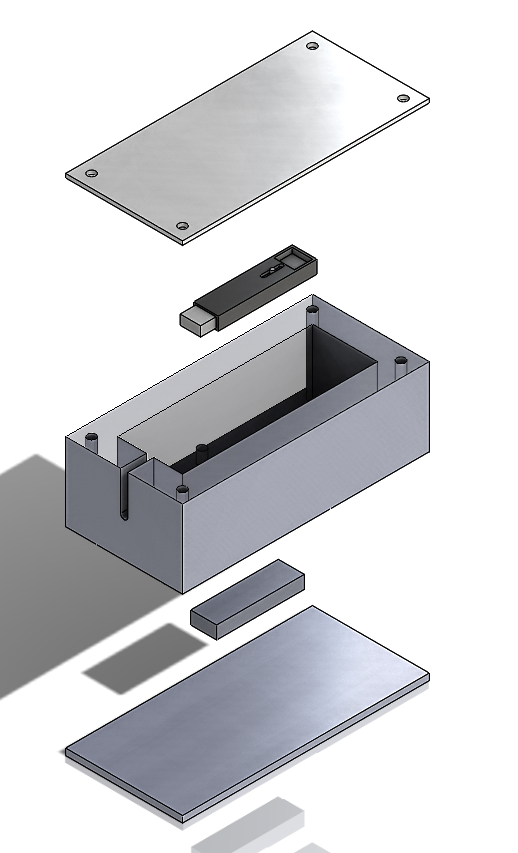
\includegraphics[width=0.5\textwidth]{figures/fitpix-case-exploded.png}
		\caption{Exploded view of the FITPix case assembly.}
		\label{fig:fitpix-container}
	\end{center}
\end{figure}

% Section for the MiniPIX configuration (including figure(s))
As previously mentioned, the MiniPIX was placed within the mock-up ISS module.
The module was constructed using the materials and material proportions given by Ref. \cite{NASA-ISS-Construction}.
The description of the module layers can be seen in Figure \ref{fig:iss-module}.
Aluminum 2219-T87 is aircraft grade material, is very expensive (on the order of several thousand dollars), and can only be ordered in bulk.
Due to monetary constraints, it was replaced with aluminum 6061-T6, but the dimensions were kept the same.
% Manufacturing the ISS module
%The ISS module was constructed layer by layer.
The inner-most (atmosphere-containing) aluminum structure was constructed by cutting sheets for each face of the box then welding the pieces together to form the box.
%This structure was then wrapped by the kevlar fabric.
%With the thickness of the fabric ordered, 
The front face of the box was left open to allow access to the inside of the structure.
In order to simulate the ISS environment as closely as possible, the module was to be pressurized at one atmosphere.
This was to be accomplished by sealing gaps in the structure with a vacuum epoxy once the entire system was assembled.
To measure pressure and temperature inside the module, a sensor was placed inside with wires fed through the layers and sealed with epoxy.

\begin{figure}[h!]
	\begin{center}
		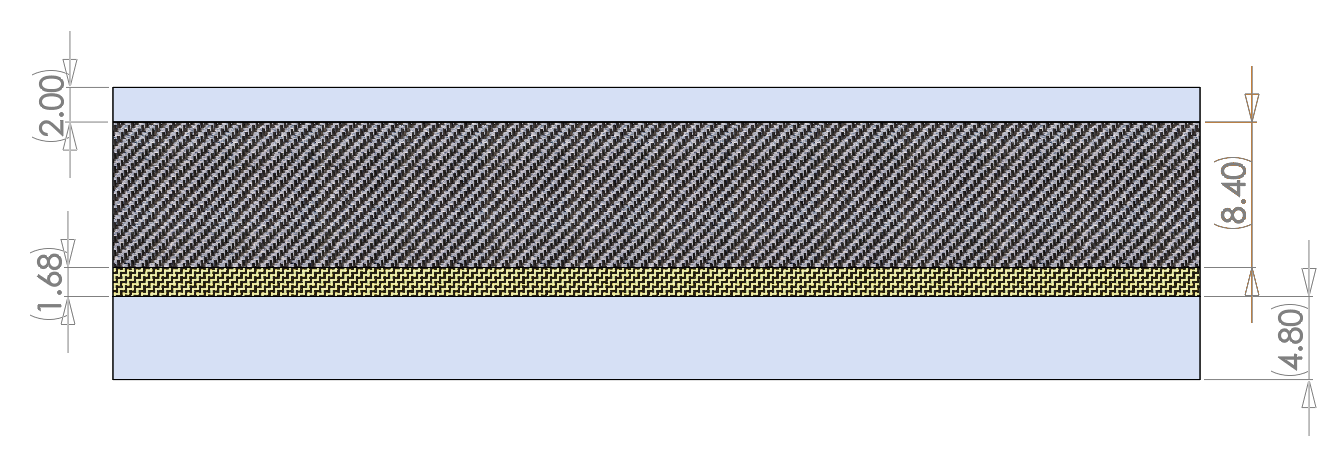
\includegraphics[width=\textwidth]{figures/iss_cross_section.png}
		\caption{Layers and thicknesses of the materials that will be used to construct the ISS module. From top to bottom: aluminum 6061-T6, six layers of Nextel AF62, six layers of Kevlar fabric, and aluminum 2219-T87. The atmosphere is contained by the 4.8 mm layer of aluminum. All dimensions are in mm.}
		\label{fig:iss-module}
	\end{center}
\end{figure}

\subsubsection{Organic Solar Cells}
